\documentclass[a4paper,10pt,brazilian]{article}
\usepackage[brazilian]{babel}
\usepackage[T1]{fontenc}
\usepackage{ae}
\usepackage[utf8]{inputenc}

\usepackage{amssymb}
\usepackage{amstext}
\usepackage{amsmath}

\usepackage{enumerate}
\usepackage{color}
\usepackage{graphicx}

\title{INF2914 - Metaeurísticas \\ Desafio de Problemas Clássicos}
\author{Pedro Teixeira}

\begin{document}
\maketitle

\section{O Problema}

Escolhi abordar o Problema de \textbf{Steiner} em Grafos para o desafio da disciplina, basicamente por dois motivos: por ser um dos mais famosos dos quais eu não conhecia nada, e pelo fato de ser um problema em \textbf{grafos}. Durante as aulas da disciplina tive a oportunidade de trabalhar com metaheurítiscas para os problemas do TSP e do QAP que podem ser representados apenas por uma permutação e queria experimentar com algo diferente.

\section{As instâncias e os resultado}

As duas instâncias do desafio \textit{steiner-1-2353.stp} (ALUT1181) e \textit{steiner-2-3413.stp} (ALUE5623) foram resolvidas nos valores propostos, inclusive alcançando os \textbf{valores ótimos} para ambas. Lembrando que ALUE5623 é classificada na steinlib com dificuldade NP\footnote{\textit{No polynomial time algorithm is known. Use of an exponential time enumeration sceme like Branch-and-Bound is neccessary.}}.

A solução foi implementada, no período aproximado de uma semana, e esse breve relatório tem o objetivo de ilustrar os resultados obtidos e mencionar as técnicas utilizadas.

\section{Resolvendo o problema}

\subsection{Visão inicial e decepções}
A estratégia inicial era: testar Simulated Annealing com alguma vizinha de troca de vértice ou aresta. Se não der certo, tentar algo com Ant System.

Para construção de uma solução viável usei a heurística de cheapest insert(CHINS) de Takahashi e Matsuyama conforme explicada nesta tese de mestrado\cite{tabu}.

Porém, logo percebi que com o SA e uma vizinhança simples de troca aleatória não iria me levar nem próximo ao valor do desafio - apenas \textit{modificar} soluções e aceitar soluções ruins sem nenhum fator de restrição não era eficiente. Durante todo os experimentos com o SA, os valores nunca era melhores do que a construção inicial o que foi realmente frustrante.

Para fortalecer a busca por melhor qualidade, implementei a vizinhança baseada em caminhos, onde \textit{key-paths} são substituídos pelo caminho mais curto do grafo original. Mesmo assim, ela chegava apenas no mesmo valor da construção inicial, que era um ótimo local. Neste momento, estava ainda, inocentemente, escolhendo o mesmo terminal como raíz.

\section{Bugs, C++ e Boost}

Mesmo não sendo minha linguagem de programação mais fluente, optei por implementar em C++ (com Eclipse utilizando g++ no Ubuntu 8.04) e com intuito de agilizar o desenvolvimento, procurei alguma biblioteca com as estruturas de dados e algorítmos para grafos. Boost pareceu ser a mais ampla, flexivel e professional de todas que pesquisei - logo foi a escolhida. Porém a curva de aprendizado foi maior que atencipei e durante 60\% do tempo de desenvolvimento foi gasto aprendendo a utilizar a API e corrigido de mal uso das estruturas e algoritmos com o  auxílio do valgrind\footnote{Valgrind é uma excelente ferramenta para trace e profiling em c++ para linux.}. 

De qualquer forma, preciso enfatizar aqui que Boost é excelente e (mesmo sendo difícil de aprender) vale a pena\footnote{Algorítmo de Prim's para MST usa as complexas \textit{relaxed heaps}, que chega ser melhor que implementações com as de Fibonacci, DFS permite receber um \textit{visitor} externo, a estrutura de dados adjacency\_list é conveniente, etc..}. 

\subsection{Desespero e pré-processamento}

Com o tempo perdido em programação e o prazo chegando, pensei que algum tipo de pré-processamento seria a salvação. Consultei a literatura\cite{uchoa99preprocessing} e comecei a implementar algumas reduções simples. Porém durante algumas pesquisas, encontrava mais referências a heurísticas de construções e quando encontrei estes trabalhos de busca local\cite{Poggi_hybridlocal} e de GRASP, decidi tentar as idéias descritas neles.

Caso, mesmo assim, não tive sucesso iria tentar implementar a heurística de Robins e Zelikowsky(2001) que tem o melhor ratio (de 1.55) de todos os algoritmos aproximados. 

\subsection{Boas Heurísticas}

Não foi necessário ir muito longe. Com os problemas de programação resolvido, uma construção aleatórizada com uma busca por \textit{key-node} foi suficiente para atingir valores ótimos muito rápido. Para cada solução, tentamos incluir cada \textit{key-node} na construção inicial (onde um vértice é escolhido aleatóriamente como raíz) até melhorarmos. 

Não foi nem necessário aplicarmos busca local baseada em troca de key-path.

\section{Resultados}

Os valores com a heurística de busca local de inserção de key-nodes:

\begin{tabular}{|c|c|c|c|c|}
\hline  Instância & Valor  & Tempo(s)  & \#iterações & OPT  \\ 
\hline  steiner-1 &  2353 &  95 & 750 & 2353 \\ 
\hline  steiner-2 &  3413 &  678 & 2850 & 3413  \\ 
\hline 
\end{tabular} 

Para cada uma, segue um gráfico de variação de valores durante a execução da busca local.

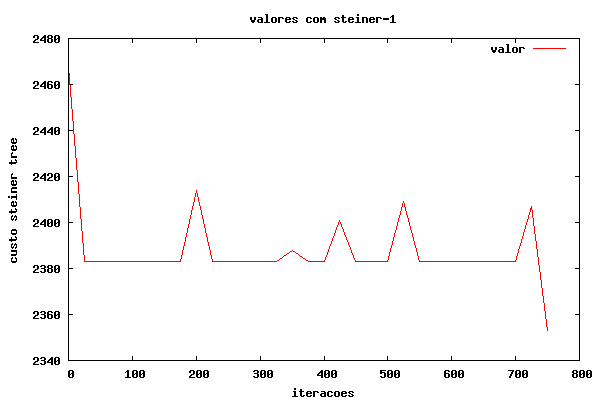
\includegraphics[scale=0.5]{1graph.png} 

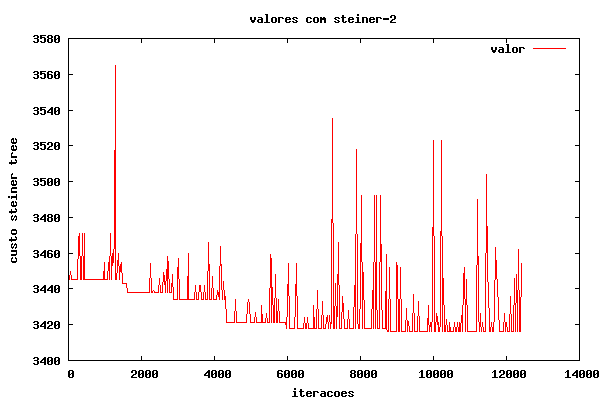
\includegraphics[scale=0.5]{2graph.png} 

\section{Conclusão e futuro}

Aprendi muito com este trabalho. Não só sobre steiner e suas heurísticas, mas muita coisa sobre c++, algoritmos e estrutura de dados para teoria de grafos. Apesar de indo quase a loucura no início, foi gratificante no final.

Com essa experiência, perdi uma certa inocência que tinha em relação a problemas de otimização, e foi muito bom ter a pressão de um desafio para por a mão na massa. E além de tudo, foi uma grata surpresa descobrir que o meu professor (com outros pesquisadores brasileiros) é autor de quase todos os artigos relevantes para resolução do Problema de Steiner em Grafos.

Como trabalho futuro, fiquei muito interessado em ter algum motivo para implementar a heurística\cite{1071708} que usa contração de vértices e tem o melhor bound garantido até então.

\bibliography{references}{}
\bibliographystyle{plain}


\end{document}